\documentclass{report}
\usepackage{mathtools}
\usepackage{color}
\title{Projet d’Analyse Syntaxique Université de Bordeaux, année 2014–2015 L3 Informatique et Math-Info.}
\begin{document}
\maketitle
\tableofcontents
\part{Introduction}
\part{Projet}
\paragraph{bleu}{\color{blue}blue test this is a test }
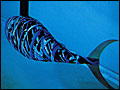
\includegraphics{pic.jpg}
\chapter{Présentation du Projet}
\chapter{Objectifs Atteints}
\chapter{Présentation du code C}
\chapter{Présentation de la documentation}
\chapter{Avis Personnel}
\part{Conclusion}
\end{document}
